%---------- Inleiding ---------------------------------------------------------

% TODO: Is dit voorstel gebaseerd op een paper van Research Methods die je
% vorig jaar hebt ingediend? Heb je daarbij eventueel samengewerkt met een
% andere student?
% Zo ja, haal dan de tekst hieronder uit commentaar en pas aan.

%\paragraph{Opmerking}

% Dit voorstel is gebaseerd op het onderzoeksvoorstel dat werd geschreven in het
% kader van het vak Research Methods dat ik (vorig/dit) academiejaar heb
% uitgewerkt (met medesturent VOORNAAM NAAM als mede-auteur).
% 

\section{Inleiding}%
\label{sec:inleiding}

Het efficiënt beheren van gegevens en bestanden wordt steeds belangrijker voor organisaties, 
inclusief kleinere organisaties zoals sportclubs. Aquarius Zwemclub Lebbeke (AZL) maakt momenteel 
gebruik van Dropbox om bestanden te delen tussen lesgevers, maar er zijn verschillende problemen. 
De toegangsrechten zijn niet altijd actueel, er is geen integratie met zowel de WordPress-website als de webapplicatie, en sommige 
lesgevers hebben geen Dropbox-account, waardoor ze geen toegang hebben tot de cloudomgeving. 
Dit leidt tot extra handmatig werk voor de beheerders.

Dit onderzoek richt zich op het vinden van een geschikt alternatief voor Dropbox dat beter aansluit 
bij de behoeften van AZL. Het doel is om een cloudopslagoplossing te vinden die eenvoudig te beheren is, 
die zorgt voor duidelijke en up-to-date toegangsrechten, en die goed integreert met de huidige systemen van de zwemclub. 
Dit zal het voor lesgevers makkelijker maken om toegang te krijgen tot de juiste bestanden en mappen, en tegelijkertijd de 
administratieve werklast voor de beheerders verlagen.

De centrale vraag in dit onderzoek is: \textit{Hoe kan AZL een cloudopslagoplossing implementeren die zorgt voor een beter beheer van de 
toegang tot bestanden, eenvoudig integreert met de bestaande systemen, en gebruiksvriendelijk is voor alle lesgevers, zonder dat zij hiervoor 
een extra account hoeven aan te maken?} Om deze vraag te beantwoorden, worden de volgende deelvragen onderzocht:
\begin{itemize}
    \item Wat zijn de mogelijkheden om een geschikte cloudopslagoplossing te voorzien?
    \item Wat zijn de voor- en nadelen van de verschillende oplossingen die beschikbaar zijn?
    \item Hoe kan elke mogelijke oplossing worden geïntegreerd met de bestaande systemen van AZL?
    \item Hoe kan het beheer van de toegang tot bestanden zo efficiënt en gebruiksvriendelijk mogelijk worden ingericht?
    \item Wat is de kostprijs van de verschillende oplossingen, en hoe verhoudt deze zich tot het budget van AZL?
\end{itemize}
Deze deelvragen vormen samen een gestructureerde aanpak om de centrale vraag te beantwoorden en een passende cloudopslagoplossing 
te vinden die aansluit bij de specifieke noden van de zwemclub.

Het doel van dit onderzoek is om verschillende cloudopslagoplossingen te vergelijken, de voor- en nadelen van elke oplossing te evalueren en uiteindelijk een werkend prototype (proof of concept) te ontwikkelen van de beste oplossing voor AZL. Het resultaat zal niet alleen een proof of concept bevatten, maar ook concrete aanbevelingen voor de implementatie van de gekozen oplossing.

%---------- Stand van zaken ---------------------------------------------------

\section{Literatuurstudie}%
\label{sec:literatuurstudie}

\subsection{Huidige IT-infrastructuur bij AZL}
Aquarius Zwemclub Lebbeke (AZL) maakt momenteel gebruik van een eenvoudige maar doeltreffende IT-infrastructuur:
\begin{itemize}
    \item \textbf{Hosting}: De WordPress-website en een webapplicatie gebouwd met Angular en Node.js zijn gehost op DigitalOcean.
    \item \textbf{E-mailservices}: De SMTP-server wordt gehost bij AWS, dit omdat deze functionaliteit niet beschikbaar is bij DigitalOcean.
    \item \textbf{Cloudopslag}: Voor het delen van bestanden tussen lesgevers wordt Dropbox gebruikt.
    \item \textbf{Authenticatie en autorisatie}: De webapplicatie maakt gebruik van een zelfgebouwd authenticatiesysteem, er wordt dus geen gebruik gemaakt van externe diensten.
\end{itemize}
Hoewel deze infrastructuur functioneel is, kent AZL verschillende uitdagingen: er is geen integratie tussen de cloudopslag en de 
WordPress-website of webapplicatie, en geautomatiseerd toegangsbeheer ontbreekt. Een complete oplossing kan deze problemen aanpakken 
door integratie tussen de cloudopslag en de applicaties mogelijk te maken, wat zal zorgen voor een gebruiksvriendelijkere en efficiëntere werking.

\subsection{Vergelijking van cloudopslagoplossingen}
Om een geschikte cloudopslagoplossing voor AZL te vinden, zijn verschillende cloudoplossingen beoordeeld op basis van criteria die specifiek aansluiten bij de uitdagingen en behoeften van de organisatie:
\begin{itemize}
    \item Geschikt zijn voor kleine tot middelgrote organisaties: De oplossing moet betaalbaar en beheersbaar zijn voor een sportvereniging met beperkte middelen.
    \item Naadloos geïntegreerd kunnen worden: De oplossing moet aansluiten op de bestaande WordPress-website en Angular-webapplicatie.
    \item Flexibel zijn in toegangsbeheer: De oplossing moet een efficiënte en veilige manier bieden om toegangsrechten te beheren, waarbij lesgevers eenvoudig kunnen worden toegevoegd of verwijderd.
    \item Gebruiksvriendelijk en technisch haalbaar zijn: De oplossing moet eenvoudig te gebruiken zijn voor lesgevers met beperkte technische kennis en flexibel genoeg voor de webmaster.
    \item Onderhoudsvriendelijk zijn: De oplossing moet eenvoudig te beheren zijn door de webmaster na de implementatie.
\end{itemize}

\subsubsection{Dropbox}
Hoewel Dropbox een gebruiksvriendelijke oplossing biedt voor het delen van bestanden, voldoet het niet aan alle behoeften van AZL. 
Het gebrek aan integratie met de bestaande systemen zorgt voor extra werk voor de beheerders, en het ontbreken van geautomatiseerd 
toegangsbeheer maakt het moeilijk om de juiste rechten op elk tijdstip te garanderen voor alle gebruikers. Bovendien vereist Dropbox dat 
elke gebruiker een account aanmaakt, wat een extra drempel kan vormen voor lesgevers die niet vertrouwd zijn met de dienst.

Dropbox biedt via de Dropbox API de mogelijkheid om cloudopslagfunctionaliteiten, zoals bestandenbeheer en mappenbeheer, in webapplicaties te integreren \autocite{dropbox_api}. 
De API stelt ontwikkelaars in staat om bestanden te uploaden, downloaden, mappen te creëren en bestanden te delen, wat ideaal lijkt voor het delen van 
bestanden tussen lesgevers bij Aquarius Zwemclub Lebbeke (AZL). Echter, de meeste van deze functies vereisen het gebruik van OAuth 2.0 voor de authenticatie 
en autorisatie van gebruikers \autocite{dropbox_oauth}.

De webapplicatie voor de lesgevers bij AZL maakt geen gebruik van OAuth 2.0 voor authenticatie. Dit betekent dat, in de huidige opzet van de applicatie, 
het technisch niet eenvoudig is om gebruikers veilig toegang te geven tot hun Dropbox-accounts zonder dat hun inloggegevens gedeeld worden. Om Dropbox te 
integreren, zou het volledige authenticatiesysteem van de applicatie moeten worden omgebouwd om OAuth 2.0-ondersteuning toe te voegen \autocite{dropbox_oauth}. Dit houdt in dat de 
applicatie de benodigde infrastructuur moet opzetten om gebruikers via OAuth 2.0 te authenticeren, wat een significante verandering in het huidige systeem vereist.

Zonder OAuth 2.0 zou de applicatie afhankelijk moeten zijn van andere methoden om verbinding te maken met Dropbox, zoals het handmatig verstrekken van API-sleutels 
of toegangstokens. Deze benadering is echter niet aanbevolen, omdat het in strijd is met moderne beveiligingspraktijken. Het ontbreken van OAuth 2.0 betekent 
dat de applicatie niet de benodigde bescherming kan bieden voor gebruikersgegevens, waardoor de vertrouwelijkheid en de integriteit van opgeslagen bestanden 
in gevaar komen.

Daarnaast is de opslagcapaciteit van een gratis persoonlijk Dropbox-account beperkt tot 2 GB, wat mogelijk onvoldoende is voor de toekomstige behoeften van AZL, 
vooral wanneer meerdere gebruikers bestanden moeten delen en opslaan. Het beheer van gebruikersmappen en het toekennen van individuele toegang tot deze 
mappen is ook problematisch, omdat de API geen methode biedt om toegang per gebruiker te regelen zonder OAuth 2.0.

Gezien de beperkingen van een gratis persoonlijk Dropbox-account, het ontbreken van OAuth 2.0-authenticatie, en de noodzaak om het gehele authenticatiesysteem 
om te bouwen, is de integratie van Dropbox in de webapplicatie voor lesgevers technisch haalbaar, maar het vereist aanzienlijke aanpassingen aan de infrastructuur 
en beveiligingsstructuur van de applicatie.

\subsubsection{Amazon S3}
Amazon S3 (Simple Storage Service) is een populaire cloudopslagoplossing die bekend staat om zijn schaalbaarheid, betrouwbaarheid en hoge beschikbaarheid. Het biedt objectopslag voor het opslaan van gegevens in de cloud, waarbij elk bestand (object) is opgeslagen in een zogenaamde "bucket". S3 biedt een uitgebreide set van API's die kunnen worden gebruikt om gegevens te beheren, inclusief de mogelijkheid om bestandsbeveiliging in te stellen, versiebeheer toe te passen, en gegevens te repliceren naar verschillende regio's voor redundantie \autocite{aws_s3}. Amazon S3 biedt ook integratie met andere AWS-diensten, wat het geschikt maakt voor organisaties die andere AWS-diensten gebruiken.

Een belangrijk voordeel van Amazon S3 is de flexibiliteit bij het instellen van toegangscontrole via IAM (Identity and Access Management), waarmee gedetailleerde machtigingen kunnen worden ingesteld voor gebruikers en toepassingen \autocite{aws_iam}. Voor AZL zou dit het mogelijk maken om de toegang tot verschillende bestanden of mappen eenvoudig te beheren op basis van de rol van de gebruiker binnen de organisatie.

Echter, de prijsstructuur van Amazon S3 kan complex zijn, afhankelijk van factoren zoals het aantal opgeslagen gegevens en het aantal verzoeken, wat kan leiden tot hogere kosten naarmate de opslagbehoeften groeien \autocite{aws_pricing}. Dit kan een belangrijke overweging zijn voor kleinere organisaties zoals AZL, die mogelijk een goedkopere oplossing nodig hebben.

\subsubsection{Nextcloud}
Nextcloud is een open-source cloudopslagoplossing die bekend staat om zijn flexibiliteit en controle over gegevens. Het biedt een privé cloudopslagplatform dat bedrijven in staat stelt om hun eigen infrastructuur te gebruiken voor het hosten van hun gegevens, in plaats van afhankelijk te zijn van externe providers. Nextcloud ondersteunt integraties met externe diensten zoals Dropbox, Google Drive en Amazon S3, en biedt uitgebreide mogelijkheden voor bestandssynchronisatie en delen \autocite{nextcloud_features}.

Voor AZL zou Nextcloud de mogelijkheid bieden om de volledige controle over hun gegevens te behouden, aangezien het lokaal gehost kan worden of via een gehoste oplossing kan worden gebruikt. Het biedt ook een uitgebreid systeem voor toegangsbeheer, inclusief ondersteuning voor single sign-on (SSO) en federated cloud, waarmee bestanden veilig tussen verschillende instellingen kunnen worden gedeeld \autocite{nextcloud_sso}. Daarnaast biedt Nextcloud een API waarmee de cloudopslag eenvoudig kan worden geïntegreerd met andere applicaties, wat de interoperabiliteit met de bestaande systemen van AZL vergemakkelijkt.

Een ander voordeel van Nextcloud is de mogelijkheid om de kosten te beheersen, aangezien het open-source is en zonder licentiekosten kan worden geïmplementeerd. Er kunnen echter kosten ontstaan bij het hosten van de serverinfrastructuur en het onderhouden van de software. Ook moet de juiste technische expertise aanwezig zijn om de oplossing op te zetten en te beheren.

\subsubsection{Microsoft Azure}
Microsoft Azure biedt een breed scala aan cloudopslagoplossingen, waaronder Blob Storage voor objectopslag, File Storage voor bestandsgebaseerde opslag, en Disk Storage voor virtuele machines. Azure Blob Storage biedt een schaalbare en betrouwbare oplossing voor het opslaan van grote hoeveelheden ongestructureerde data, wat het geschikt maakt voor het beheren van bestanden zoals documenten, afbeeldingen en video's \autocite{azure_blob}.

Azure biedt ook uitgebreide integratiemogelijkheden, waaronder een sterk toegangsbeheer met Azure Active Directory (AD), wat het voor AZL mogelijk maakt om naadloos toegang te verlenen tot opslag op basis van gebruikersrollen en organisatorische vereisten \autocite{azure_ad}. Daarnaast maakt Azure gebruik van wereldwijde datacenters, waardoor het platform hoge beschikbaarheid en redundantie biedt.

Een potentieel nadeel van Azure is de prijsstelling, die op basis van gebruik kan variëren, wat moeilijk voorspelbaar kan zijn voor kleinere organisaties zoals AZL. De complexiteit van de dienst kan ook een uitdaging zijn voor organisaties die geen uitgebreide IT-afdeling hebben \autocite{azure_pricing}.

\subsubsection{Google Cloud Storage}
Google Cloud Storage biedt schaalbare en betrouwbare opslag voor een breed scala aan gegevens, van ongestructureerde data tot back-ups en archivering. Het biedt een eenvoudig te gebruiken API voor het uploaden, downloaden en beheren van bestanden \autocite{google_storage}. Google Cloud Storage heeft ook geavanceerde beveiligingsfuncties, zoals encryptie van gegevens in rust en tijdens overdracht, en uitgebreide toegangscontrole via Google Cloud Identity and Access Management (IAM) \autocite{google_iam}.

Een belangrijk voordeel van Google Cloud Storage is de sterke integratie met andere Google-diensten zoals Google Drive, Firebase en BigQuery, wat de interoperabiliteit met andere systemen vergemakkelijkt. Voor AZL zou Google Cloud Storage een gebruiksvriendelijke oplossing kunnen bieden, met robuuste beveiligingsmaatregelen en een sterke focus op prestaties.

Net als bij andere grote cloudproviders, is de prijsstructuur van Google Cloud Storage complex, en de kosten kunnen oplopen naarmate de opslagbehoeften van AZL groeien \autocite{google_pricing}. De schaalvoordelen van Google kunnen echter voordelig zijn voor grotere organisaties, terwijl kleinere organisaties mogelijk baat hebben bij alternatieven zoals Nextcloud of DigitalOcean Spaces.

\subsubsection{DigitalOcean Spaces}
DigitalOcean Spaces biedt een eenvoudige en kosteneffectieve oplossing voor objectopslag in de cloud. Het is specifiek ontworpen voor ontwikkelaars en kleinere organisaties die op zoek zijn naar een flexibele en gebruiksvriendelijke oplossing voor het beheren van bestanden en gegevens \autocite{digitalocean_spaces}. DigitalOcean biedt ook een eenvoudige API en integratie met hun andere cloud-diensten, zoals databases en virtuele machines.

Een voordeel van DigitalOcean Spaces is de eenvoudige prijsstelling, die transparant en voorspelbaar is, wat het geschikt maakt voor kleinere organisaties zoals AZL. Het platform is echter beperkter in functionaliteit vergeleken met grotere providers zoals AWS of Google Cloud, wat het minder geschikt maakt voor complexe of grootschalige toepassingen \autocite{digitalocean_pricing}.





%---------- Methodologie ------------------------------------------------------
\section{Methodologie}%
\label{sec:methodologie}
\subsection{Fase 1: Literatuurstudie}
In deze fase wordt een literatuurstudie uitgevoerd om een overzicht te krijgen van de beschikbare cloudopslagoplossingen en hun mogelijkheden. De focus ligt op het identificeren van oplossingen die geschikt zijn voor kleinere organisaties zoals Aquarius Zwemclub Lebbeke (AZL), met specifieke aandacht voor integratie met bestaande systemen, toegangsbeheer, beveiliging en kosteneffectiviteit. De resultaten van deze literatuurstudie zullen worden gebruikt om een longlist van mogelijke cloudopslagoplossingen op te stellen, die in de volgende fase verder zullen worden onderzocht.

\subsection{Fase 2: Requirements verzamelen}
In deze fase wordt de focus gelegd op het verzamelen van de vereisten voor een nieuwe cloudopslagoplossing voor Aquarius Zwemclub Lebbeke (AZL). Gezien de aard van de bestaande problemen met de huidige Dropbox-implementatie, wordt er voornamelijk samengewerkt met de webmaster, die verantwoordelijk is voor het beheer van de gedeelde mappen. Dit zorgt voor een gedetailleerd inzicht in de huidige knelpunten en de behoeften van de club met betrekking tot cloudopslag.

Het doel van deze fase is om zowel functionele als niet-functionele eisen in kaart te brengen voor de cloudopslagoplossing die moet worden geïntegreerd met de bestaande infrastructuur, waaronder de WordPress-website en de webapplicatie voor lesgevers (gebaseerd op Angular en Node.js). Belangrijke vraagstukken die moeten worden onderzocht zijn onder andere:
\begin{itemize}
    \item \textbf{Toegangsbeheer}: Hoe kan toegang tot de cloudopslag op een efficiënte en veilige manier worden geregeld voor de verschillende lesgevers? Er moet worden nagedacht over wie toegang krijgt en hoe dit dynamisch kan worden aangepast naargelang de status van de lesgevers (bijvoorbeeld wanneer zij stoppen of tijdelijk geen toegang nodig hebben).
    \item \textbf{Beveiliging en privacy}: Hoe kunnen we ervoor zorgen dat lesgevers enkel toegang hebben tot de bestanden en mappen die voor hen relevant zijn, zonder dat andere informatie toegankelijk is?
    \item \textbf{Integratie met bestaande systemen}: Kan de nieuwe oplossing naadloos worden geïntegreerd met de bestaande webapplicatie voor lesgevers of de publieke website van de zwemclub? Dit omvat zowel technische integratie als gebruikersgemak.
    \item \textbf{Kosten}: Wat zijn de kosten van de nieuwe oplossing en hoe verhouden deze zich tot de huidige Dropbox-oplossing (gratis)? Dit kan de keuze voor bepaalde cloudopslagoplossingen beïnvloeden.
    \item \textbf{Beheer en onderhoud}: Hoe kan de oplossing eenvoudig worden beheerd door de webmaster en andere betrokkenen, en welke ondersteuning is nodig om te zorgen voor een duurzame implementatie?
\end{itemize}

Tijdens deze fase zal ook de MoSCoW-methode worden toegepast om de prioriteiten te bepalen, waarbij de belangrijkste vereisten worden gemarkeerd als ‘Must Have’, gevolgd door ‘Should Have’, ‘Could Have’, en ‘Won’t Have’. Het resultaat van deze fase zal een gedetailleerde lijst van vereisten zijn, inclusief prioriteitstelling, die als basis zal dienen voor de verdere ontwikkeling van de cloudopslagoplossing.

\subsection{Fase 3: Long list van mogelijke cloudoplossingen}
In deze fase wordt een uitgebreide lijst van mogelijke technologische oplossingen en alternatieven (long list) opgesteld. Dit gebeurt door middel van een literatuuronderzoek en het verkennen van bestaande software en systemen voor cloudopslag en documentbeheer die voldoen aan de specifieke behoeften van Aquarius Zwemclub Lebbeke (AZL). Het doel is om een breed scala aan mogelijke oplossingen te onderzoeken, waarbij geen alternatieven worden uitgesloten, zodat alle opties overwogen kunnen worden.

AZL gebruikt op dit moment Dropbox voor gedeelde mappen, maar dit brengt diverse problemen met zich mee. Zo vergeten lesgevers vaak dat deze mappen bestaan, hebben niet de juiste rechten, of kunnen er niet bij zonder Dropbox-account. Om deze redenen richt dit onderzoek zich op het vinden van alternatieve cloudoplossingen die eenvoudig geïntegreerd kunnen worden met AZL’s bestaande webapplicatie voor lesgevers (ontwikkeld in Angular en Node.js) of de publieke WordPress-website. Belangrijke selectiecriteria zijn onder andere gebruiksvriendelijkheid, efficiënt toegangsbeheer, beveiligingsopties en kosteneffectiviteit.
\subsection{Fase 4: Short list}
In deze fase wordt een selectie gemaakt uit de eerder opgestelde longlist met mogelijke technologische oplossingen. De selectie gebeurt op basis van een vergelijkende analyse waarin de alternatieven worden beoordeeld aan de hand van de criteria opgesteld in fase 2, zoals efficiënt toegangsbeheer, integratie met de bestaande webapplicatie en de WordPress-website, beveiliging en kosten. Een samenvattende tabel vat de voor- en nadelen van elk alternatief samen, wat helpt om de systemen te identificeren die het beste aansluiten bij de specifieke behoeften van AZL. De alternatieven die het meest veelbelovend zijn op het gebied van functionaliteit, veiligheid en kostenbesparing worden geselecteerd voor verder onderzoek in de volgende fase.
\subsection{Fase 5: Proof of Concept (PoC)}
In deze fase wordt een Proof of Concept (PoC) ontwikkeld om te testen of de geselecteerde oplossing daadwerkelijk in staat is de huidige problemen binnen AZL op te lossen. De PoC bestaat uit een werkend prototype van de cloudopslagoplossing, dat als feature wordt geïntegreerd in de bestaande webapp of publieke website. Na het maken van de PoC wordt deze gedurende 2 weken getest door de webmaster en lesgevers om te controleren of de oplossing voldoet aan de gestelde eisen en verwachtingen. Na deze testperiode wordt de feedback van de gebruikers verzameld en geanalyseerd om eventuele verbeteringen aan te brengen in de PoC. Het doel van deze fase is om te valideren of de geselecteerde oplossing daadwerkelijk een verbetering is ten opzichte van de huidige Dropbox-implementatie en om te bepalen het onderzochte alternatief daadwerkelijk geschikt is voor implementatie binnen AZL.
\subsection{Fase 6: Evaluatie en conclusies}
Na de implementatie van het Proof of Concept volgt een grondige evaluatie van de resultaten. De focus ligt op de effectiviteit van de oplossing en in hoeverre deze de problemen rondom het documentbeheer en toegangsbeheer van AZL oplost. Eventuele tekortkomingen of beperkingen worden gedocumenteerd, en verbeterpunten worden geïdentificeerd om de oplossing verder te optimaliseren.

Op basis van de evaluatie worden conclusies getrokken en aanbevelingen gedaan voor de implementatie van de oplossing binnen AZL.
\subsection{Visualisatie en Tijdsplanning}
De onderstaande Gantt Chart biedt een visueel overzicht van de tijdsplanning voor mijn bachelorproef, die loopt van 07/03/2025 tot 23/05/2025. De chart geeft een gedetailleerd overzicht van de verschillende fasen van het project, waarbij elke fase zorgvuldig is ingepland om een optimale voortgang te garanderen.

De tijdsplanning is opgedeeld in zes fasen: Literatuurstudie, Requirements verzamelen, Long list van mogelijke cloudoplossingen, Short list, Proof of Concept (PoC) en Evaluatie en conclusies. Elke fase bouwt voort op de voorgaande, zodat er een gestructureerde aanpak wordt gevolgd die resulteert in een gedegen eindresultaat.

In de eerste fasen wordt de focus gelegd op onderzoek en analyse, terwijl in de latere fasen praktische implementatie, testen en evaluatie centraal staan. De Gantt Chart weerspiegelt deze opbouw en toont de tijdsduur die aan elke fase is toegewezen, zodat de voortgang en deadlines helder zichtbaar zijn.
\begin{figure}[h!]
    \centering
    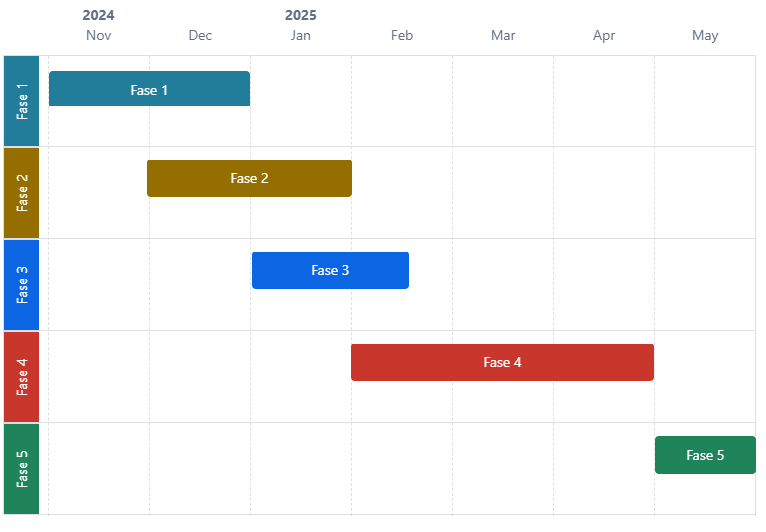
\includegraphics[width=.5\textwidth]{../graphics/Chart-Tijd-Visualisatie.png}
    \caption{Tijdsplanning van het project}
    \label{fig:tijdsplanning}
\end{figure}


%---------- Verwachte resultaten ----------------------------------------------
\section{Verwacht resultaat, conclusie}%
\label{sec:verwachte_resultaten}

De meerwaarde van deze bachelorproef voor de doelgroep, de Aquarius Zwemclub Lebbeke, is duidelijk: de implementatie van een robuuste cloudopslagoplossing zal niet alleen de werkprocessen voor de lesgevers verbeteren, maar ook de algehele efficiëntie van de club vergroten. Door de administratieve processen te automatiseren en beter beheersbaar te maken, wordt er tijdswinst geboekt, wat meer ruimte biedt voor de daadwerkelijke activiteiten van de club. Bovendien zal de verbetering van de toegang en beveiliging van documenten bijdragen aan een professionelere werking van de zwemclub.

De verwachte conclusie van deze bachelorproef is dan ook dat het gekozen cloudopslagsysteem zowel technisch haalbaar als praktisch effectief zal zijn voor de behoeften van de zwemclub. Mocht de gekozen oplossing echter niet voldoen aan de verwachtingen, dan zal het onderzoek zich richten op het identificeren van de tekortkomingen en de redenen waarom deze oplossing niet geschikt bleek. In dat geval zal er verder onderzocht worden welke alternatieven nog beter aansluiten bij de eisen van AZL.